%% IEEE Access Supplementary Material for the article in main.tex. It prints
%% the shared appendices (../appendix.tex), which the article leaves out so
%% that it stays under the 20 pages IEEE Access recommends (submission
%% checklist, item 17: "Additional content can be added as supplementary
%% material"). Same template and preamble as the article (main.tex; keep the
%% two in step). Appendices keep their letters, tables and figures are
%% numbered S1, S2, ..., and xr-hyper reads main.aux, so labels of the article
%% resolve here ("Section V-B" or "Table 2" means the article's) and citations
%% carry the article's reference numbers.
%%
%% Build: pnpm build:paper:ieee (the article and this supplement read each
%% other's .aux, so the target builds them in turn until both settle).
\documentclass{ieeeaccess}
\usepackage{cite}
\usepackage{amsmath,amssymb,amsfonts}
\usepackage{textcomp}
\usepackage{amsthm}
\usepackage{booktabs}
\usepackage{needspace}
\usepackage{placeins}
\newcommand{\keepheading}{\needspace{6\baselineskip}}
\newcommand{\keeprunin}{\needspace{4\baselineskip}}
\usepackage{array}
\usepackage{algorithm}
\usepackage{algorithmic}
%% The two class/pgf clashes main.tex documents, handled the same way.
\let\ieeeaccessclassyear\year
\def\year{2026}
\usepackage{pgfplots}
\pgfplotsset{compat=1.18}
\usetikzlibrary{arrows.meta, positioning, calc}
\let\year\ieeeaccessclassyear
\makeatletter
\pgfutil@addpdfresource@colorspaces{\the\PANTONE}
\makeatother
% GENERATED. Do not edit.
\newcommand{\frontierplots}{\addplot+[error bars/.cd, y dir=both, y explicit] coordinates { (0.02,0.0) +- (0,0.0) (0.05,38.6) +- (0,29.5) (0.1,82.6) +- (0,9.8) (0.2,88.1) +- (0,0.8) }; \addlegendentry{SO formatting-only} \addplot+[error bars/.cd, y dir=both, y explicit] coordinates { (0.02,0.0) +- (0,0.0) (0.05,0.0) +- (0,0.0) (0.1,55.6) +- (0,29.0) (0.2,87.4) +- (0,3.2) }; \addlegendentry{SO synonym rewording} \addplot+[error bars/.cd, y dir=both, y explicit] coordinates { (0.02,0.0) +- (0,0.0) (0.05,1.0) +- (0,8.8) (0.1,66.3) +- (0,25.1) (0.2,86.6) +- (0,3.1) }; \addlegendentry{SO scope widening} \addplot+[error bars/.cd, y dir=both, y explicit] coordinates { (0.02,0.0) +- (0,0.0) (0.05,0.0) +- (0,0.0) (0.1,8.4) +- (0,10.6) (0.2,52.1) +- (0,10.1) }; \addlegendentry{Djinni formatting-only} \addplot+[error bars/.cd, y dir=both, y explicit] coordinates { (0.02,0.0) +- (0,0.0) (0.05,0.0) +- (0,0.0) (0.1,14.4) +- (0,11.0) (0.2,48.6) +- (0,10.4) }; \addlegendentry{Djinni criteria change}}
\newcommand{\powerplots}{\addplot coordinates { (0,100.0) (0.005,99.9) (0.01,98.9) (0.02,88.7) (0.04,22.8) (0.05,5.5) (0.0525,3.5) (0.055,2.8) (0.0625,0.9) (0.08,0.2) (0.15,0.0) }; \addlegendentry{$n_j{=}600$} \addplot coordinates { (0,100.0) (0.005,99.9) (0.01,98.9) (0.02,92.0) (0.04,48.4) (0.05,9.8) (0.0525,6.2) (0.055,3.0) (0.0625,0.8) (0.08,0.1) (0.15,0.0) }; \addlegendentry{$n_j{=}1{,}800$} \addplot coordinates { (0,100.0) (0.005,99.8) (0.01,98.9) (0.02,92.5) (0.04,28.9) (0.05,2.9) (0.0525,1.1) (0.055,0.7) (0.0625,0.0) (0.08,0.0) (0.15,0.0) }; \addlegendentry{$n_j{=}5{,}000$}}

% GENERATED by scripts/experiments/gen-paper-assets.ts. Do not edit.
% Every number cited in prose is defined here from result artifacts.
\newcommand{\floorBool}{5.0\%}
\newcommand{\editFlipFreshBoth}{7.2\%}
\newcommand{\floorTrueStratum}{24.1\%}
\newcommand{\floorFalseStratum}{3.1\%}
\newcommand{\floorTrueCi}{[19.6, 28.8]}
\newcommand{\floorFalseCi}{[2.5, 3.7]}
\newcommand{\floorBoolVote}{6.30\%}
\newcommand{\floorBoolStored}{6.0\%}
\newcommand{\labelChurn}{4.8\%}
\newcommand{\flipInstrumentGapRows}{7}
\newcommand{\floorSelect}{6.5\%}
\newcommand{\floorDefaultT}{9.5\%}
\newcommand{\floorTzeroProbe}{3.0\%}
\newcommand{\flipSoFormatting}{6.3\%}
\newcommand{\flipSoSynonym}{8.90\%}
\newcommand{\flipSoWidening}{9.45\%}
\newcommand{\flipDjFormatting}{12.30\%}
\newcommand{\flipDjCriteria}{12.45\%}
\newcommand{\benchN}{2{,}000}
\newcommand{\benchSavings}{82.6\%}
\newcommand{\benchSavingsMain}{86.2\%}
\newcommand{\benchSavingsPi}{[82, 86]}
\newcommand{\benchRealizedCi}{[2.6, 4.3]}
\newcommand{\bootB}{1{,}000}
\newcommand{\benchRealized}{3.20\%}
\newcommand{\benchOracleTight}{765}
\newcommand{\benchOracleMain}{135}
\newcommand{\frontierA}{82.6\%}
\newcommand{\frontierB}{63.6\%}
\newcommand{\frontierC}{0.1\%}
\newcommand{\edgeCertRate}{0.8\%}
\newcommand{\edgeExceed}{100.0\%}
\newcommand{\sampleFracLo}{7\%}
\newcommand{\sampleFracHi}{81\%}
\newcommand{\benchOracleMean}{208}
\newcommand{\benchOracleMedian}{225}
\newcommand{\benchOracleRange}{135--405}
\newcommand{\benchOracleTightMean}{568}
\newcommand{\benchOracleTightRange}{90--765}
\newcommand{\benchOracleTightMedian}{405}
\newcommand{\reuseSetSavingsMain}{81.4\%}
\newcommand{\reuseSetSavingsTight}{8.1\%}
\newcommand{\reuseSetCertTight}{11.7\%}
\newcommand{\reuseSetDjCertMax}{0.8\%}
\newcommand{\tableConfigs}{20}
\newcommand{\certifyingConfigs}{9}
\newcommand{\ablationSavings}{61.4\%}
\newcommand{\ablationTotal}{40}
\newcommand{\ablationBetter}{1}
\newcommand{\ablationWorse}{16}
\newcommand{\aucVcacheF}{0.468}
\newcommand{\aucVcacheW}{0.499}
\newcommand{\aucInterF}{0.408}
\newcommand{\aucInterW}{0.669}
\newcommand{\simLo}{0.96}
\newcommand{\simHi}{0.99}
\newcommand{\aggFsavings}{91.0\%}
\newcommand{\aggFrealized}{5.99\%}
\newcommand{\aggFsubgroup}{36.1\%}
\newcommand{\aggWsubgroup}{44.1\%}
\newcommand{\aggWsavings}{64.0\%}
\newcommand{\aggWrealized}{9.45\%}
\newcommand{\aggTightCertF}{certifies}
\newcommand{\aggFtSavings}{28.0\%}
\newcommand{\aggFtRealized}{6.07\%}
\newcommand{\aggFtSubgroup}{45.2\%}
\newcommand{\aggTightCertW}{refuses}
\newcommand{\tauFmid}{100\%}
\newcommand{\tauFhi}{10.4\%}
\newcommand{\tauFerrLo}{4.8\%}
\newcommand{\tauFerrHi}{6.3\%}
\newcommand{\tauWmid}{99.9\%}
\newcommand{\tauWhi}{8.2\%}
\newcommand{\tauWerrLo}{8.0\%}
\newcommand{\tauWerrHi}{9.9\%}
\newcommand{\minoritySingle}{37.1\%}
\newcommand{\minorityVote}{24.7\%}
\newcommand{\minorityNoise}{20.4\%}
\newcommand{\calTrials}{396{,}000}
\newcommand{\calConfigs}{198}
\newcommand{\bThreeReuseW}{84.2\%}
\newcommand{\minZeroFlipRealized}{360}
\newcommand{\calPRange}{[0, 0.25]}
\newcommand{\calTightNulls}{54}
\newcommand{\calTightWorstCert}{0.0\%}
\newcommand{\calAlphaGrid}{0.05, 0.1, 0.2}
\newcommand{\calWorstReuseMetric}{33.3\%}
\newcommand{\calWorstP}{0.04}
\newcommand{\calWorstAlpha}{0.05}
\newcommand{\calWorstCertRate}{0.45\%}
\newcommand{\deployN}{89{,}184}
\newcommand{\deployOracle}{225}
\newcommand{\deployReused}{81{,}289}
\newcommand{\deployRecompute}{7{,}670}
\newcommand{\deploySavings}{91.1\%}
\newcommand{\deployRealized}{3.01\%}
\newcommand{\deployOverlap}{2{,}159}
\newcommand{\deployReplayMs}{4{,}257}
\newcommand{\deployTrueStratum}{7{,}715}
\newcommand{\deployCeiling}{91.3\%}
\newcommand{\deployOracleTight}{765}
\newcommand{\deploySavingsTight}{90.5\%}
\newcommand{\deployStamped}{79{,}130}
\newcommand{\deployUnstamped}{2{,}159}
\newcommand{\perCellCost}{\$0.00012}
\newcommand{\deployMatCost}{\$9.31}
\newcommand{\deployMatCells}{78{,}956}
\newcommand{\deployFreeRows}{10{,}228}
\newcommand{\deployMatHours}{7.4}
\newcommand{\deployConcurrency}{32}
\newcommand{\deployMaintCells}{7{,}895}
\newcommand{\deployMaintCost}{\$0.93}
\newcommand{\deployMaintMinutes}{43}
\newcommand{\deployAuditReleased}{1{,}807}
\newcommand{\deployAuditReleasedErr}{3.21\%}
\newcommand{\hhBudget}{135}
\newcommand{\hhSivmReused}{1{,}724}
\newcommand{\hhSivmErr}{3.36\%}
\newcommand{\hhSupgReused}{1{,}865}
\newcommand{\hhSupgErr}{6.54\%}
\newcommand{\hhSupgTrueRows}{180}
\newcommand{\hhSivmPerTest}{\delta/12}
\newcommand{\hhValuePerTest}{\delta/3}
\newcommand{\hhSivmErrW}{5.49\%}
\newcommand{\hhSupgErrW}{9.69\%}
\newcommand{\hhSupgTrueRowsW}{185}
\newcommand{\hhSivmReusedW}{1{,}621}
\newcommand{\hhSupgReusedW}{1{,}775}
\newcommand{\hhSivmReusedFrac}{86.2\%}
\newcommand{\hhSupgReusedFrac}{93.3\%}
\newcommand{\hhSivmReusedFracW}{81.0\%}
\newcommand{\hhSupgReusedFracW}{88.8\%}
\newcommand{\hhSupgSelFrac}{100.0\%}
\newcommand{\hhSupgSelFracW}{100.0\%}
\newcommand{\deployWorLoose}{0.230}
\newcommand{\deployLooseSampled}{180}
\newcommand{\deployLooseFlips}{5}
\newcommand{\deployWorLooseClears}{does not clear}
\newcommand{\deployWorTight}{0.099}
\newcommand{\deployTightSampled}{720}
\newcommand{\deployTightFlips}{25}
\newcommand{\deployWorTightClears}{clears}
\newcommand{\deployFalseStratum}{81{,}469}
\newcommand{\altModelName}{openai/gpt-5-nano}
\newcommand{\altModelFloor}{36.6\%}
\newcommand{\altModelEditFlip}{40.2\%}
\newcommand{\altModelN}{500}
\newcommand{\minZeroFlipSample}{$n^{*}{=}257$}
\newcommand{\corpusSO}{89{,}184}
\newcommand{\corpusDjinni}{210{,}250}
\newcommand{\labeledCells}{32{,}000}
\newcommand{\wideningTrueFlip}{45.7\%}
\newcommand{\wideningTrueCi}{[39.0, 52.7]}
\newcommand{\wideningTrueN}{199}
\newcommand{\boundConfigsTotal}{20}
\newcommand{\boundEbConfigs}{7}
\newcommand{\boundBetConfigs}{9}
\newcommand{\boundWorConfigs}{7}
\newcommand{\boundEbSavings}{18.5\%}
\newcommand{\boundBetSavings}{29.1\%}
\newcommand{\boundEbOracle}{11{,}515}
\newcommand{\boundBetOracle}{7{,}616}
\newcommand{\boundEbAtN}{0.144}
\newcommand{\boundBetAtN}{0.065}
\newcommand{\boundWorAtN}{0.317}
\newcommand{\boundWorSameLook}{3}
\newcommand{\boundWorLater}{4}
\newcommand{\boundWorLost}{0}
\newcommand{\boundWorExtra}{0}
\newcommand{\boundWorOracle}{12{,}325}
\newcommand{\boundWorSavings}{16.4\%}
\newcommand{\boundGapEbSavings}{18.1\%}
\newcommand{\boundGapBetSavings}{72.0\%}
\newcommand{\boundGapEbOracle}{1{,}485}
\newcommand{\boundGapBetOracle}{405}
\newcommand{\boundCalTrials}{72{,}000}
\newcommand{\boundBetNullWorst}{2.5\%}
\newcommand{\boundBetNullsOver}{0}
\newcommand{\boundNullConfigs}{18}
\newcommand{\boundEbCleanSample}{360}
\newcommand{\boundBetCleanSample}{180}
\newcommand{\totalSpend}{\$11.56}
\newcommand{\ledgerStart}{4 August 2026}
\newcommand{\ledgerEnd}{5 August 2026}
\newcommand{\famRunDate}{15 August 2026}
\newcommand{\totalCells}{98{,}496}
\newcommand{\offLedgerCells}{38{,}416}
\newcommand{\famGeminiFloor}{4.9\%}
\newcommand{\famGeminiFmt}{25.4\%}
\newcommand{\famGeminiSyn}{31.5\%}
\newcommand{\famGeminiN}{2{,}000}
\newcommand{\famGeminiFmtTrueStratum}{28.7\%}
\newcommand{\famGeminiFmtFalseStratum}{24.6\%}
\newcommand{\famGeminiFmtToFalseShare}{24.6\%}
\newcommand{\famGeminiCachedTrueShare}{21.8\%}
\newcommand{\famGeminiCaseOnlyFlip}{11.0\%}
\newcommand{\famGeminiSpaceOnlyFlip}{23.2\%}
\newcommand{\famGeminiCaseOnlyCert}{60.2\% @ 405}
\newcommand{\famGeminiSpaceOnlyCert}{refused (90)}
\newcommand{\famGeminiThreeFloor}{0.4\%}
\newcommand{\famGeminiThreeFmt}{5.8\%}
\newcommand{\famGeminiThreeN}{500}
\newcommand{\famGlmFloor}{10.3\%}
\newcommand{\famGlmFmt}{25.0\%}
\newcommand{\famGlmSyn}{31.3\%}
\newcommand{\famGlmN}{2{,}000}
\newcommand{\famGlmFmtTrueStratum}{27.0\%}
\newcommand{\famGlmFmtFalseStratum}{17.0\%}
\newcommand{\famGlmFmtToFalseShare}{86.4\%}
\newcommand{\famGlmCachedTrueShare}{80.0\%}
\newcommand{\famQwenFloor}{5.8\%}
\newcommand{\famQwenFmt}{14.6\%}
\newcommand{\famQwenN}{500}
\newcommand{\famCount}{4}
\newcommand{\famCertifying}{3}
\newcommand{\famFloorLo}{0.4\%}
\newcommand{\famFloorHi}{10.3\%}

\setlength{\emergencystretch}{2em}
\theoremstyle{definition}
\newtheorem{theorem}{Theorem}
\newtheorem{assumption}{Assumption}
%% xr-hyper imports the article's labels and its \bibcite entries, so a
%% citation carries the article's number; every key cited here must be cited
%% there too (the packager stops on an undefined citation).
\usepackage{xr-hyper}
\externaldocument{main}
\usepackage[hidelinks]{hyperref}
\hypersetup{
  pdftitle={Supplementary Material: Reuse, but Verify: Certified Maintenance of Table Cells Computed by Large Language Models under Prompt Edits},
  pdfauthor={Arjun Lohan}}
\def\UrlBreaks{\do\/}
\def\UrlBigBreaks{\do\:}
\makeatletter\mathchardef\UrlBigBreakPenalty=\@M\makeatother
\Urlmuskip=0mu

\newcommand{\sivm}{\textsc{sIVM}}
\newcommand{\secref}[1]{Section~\ref{#1}}
\newcommand{\figref}[1]{Fig.~\ref{#1}}
\newcommand{\paperroot}{..}
\newcommand{\venueappendix}{\appendices}
\newcommand{\Description}[2][]{}
\renewcommand{\thetable}{S\arabic{table}}
\renewcommand{\thefigure}{S\arabic{figure}}
\renewcommand{\theHtable}{S\arabic{table}}
\renewcommand{\theHfigure}{S\arabic{figure}}

\begin{document}
\vol{14}
\year{2026}
\markboth
{Lohan: Reuse, but Verify: Supplementary Material}
{Lohan: Reuse, but Verify: Supplementary Material}
\twocolumn[{%
\raggedright
{\color{accessblue}\titlefont Supplementary Material for ``Reuse, but
Verify: Certified Maintenance of Table Cells Computed by Large Language
Models under Prompt Edits''\par}
\vspace*{4mm}
{\authorfont\uppercase{Arjun Lohan}\par}
\vspace*{1mm}
{\addressfont University of Southern California, Los Angeles, CA, USA
(e-mail: lohan@usc.edu)\par}
\vspace*{8mm}}]

This supplement holds the appendices that the article cites by letter.
Its tables and figures are numbered S1, S2, and so on. A section,
table, figure, equation, assumption, or theorem number without the
prefix S is the article's, and citations refer to the article's
reference list.

%% Shared appendices. The preprint shell (main.tex, acmart) prints them after
%% the body; the IEEE Access shell does not, and its Supplementary Material
%% (ieee/supplement.tex) prints them instead, so the article itself stays
%% under the 20 pages IEEE Access recommends. Labels defined here are read by
%% the article through xr (ieee/main.tex), and labels of the article are read
%% here the same way (ieee/supplement.tex). Numbers remain macro-cited; the
%% guards in scripts/check-paper-numbers.ts scan this file too.
\venueappendix

\keepheading
\section{The mechanical guards}
\label{app:guards}
The checker (\texttt{scripts/check-paper-numbers.ts}) fails on any of
ten conditions.
\begin{enumerate}
\item A hand-typed quantity in the prose outside an enumerated
allow-list (user parameters such as $\alpha$ and $\delta$, protocol
constants such as the schedule looks, and generic thresholds quoted as
such).
\item A quantity hardcoded inside the generator instead of derived from
an artifact.
\item A macro defined but never cited, since an uncited macro can drift
undetected.
\item A macro whose trailing space is swallowed into the next word,
which is invisible in the source.
\item A sentence that asserts two quantities differ while citing two
macros whose values are equal.
\item A spelled-out multiplier (``twice'', ``an order of magnitude'')
that the cited macros' ratio does not support.
\item A containment claim (``inside'', ``at most'') that the cited
range and scalar macros do not support.
\item An absolute claim (``never'', ``every'', ``anywhere'') appearing
in the abstract or the contributions list without an entry in an
enumerated allow-list. This is the one class of defect the numeric
guards are blind to by construction.
\item A scope claim (``on the same column'') whose cited macros come
from different columns, checked against a provenance file the generator
emits from the same pair definitions the experiments run on.
\item A sentence of the prose, of a list item, of a caption, or of the
abstract longer than 60 words (table bodies, displayed mathematics, and
the theorem environments excluded), a readability bound.
\end{enumerate}
The generator adds guards of its own. It asserts the relations that
\secref{sec:experiments}, \secref{sec:limits}, and the appendices state
between figures: in the paragraphs on the main results, the strict
mode, the stratifier ablation, the matched competitor, the model study,
the independence check, the usable budgets, the graded relation, and
the pilot. It also asserts that the separate audit verifier reproduces
each audit the article prints, and that the released certify action is
configured as the pinned procedure. It stops if a regenerated artifact
breaks one. It rounds every figure half up on its decimal value, and
rounds upward a figure quoted as a maximum (``at most'').
Generating the quantities is necessary but not sufficient, because the
sentences that \emph{relate} quantities go stale independently of the
quantities themselves.

\FloatBarrier
\keepheading
\section{The bound ablation in detail}
\label{app:grid}
\begin{table*}[t]
\caption{Five upper confidence bounds inside the same pinned procedure
on the same stored labels. The first two columns give each bound on a
clean sample of $90$ draws and on the deployment evidence of
\deployMpFlipsLoose\ flips in \deployMpLookLoose\ draws. The four
fixed-sample bounds are read at the pinned per-look level, $\delta/12$,
and the betting sequence at the unsplit per-stratum level, $\delta/2$
(Appendix~\ref{app:grid} states the caveat on its validity). The next three columns give the certifying
configurations, mean savings, and oracle calls over the
Table~\ref{tab:main} grid (main seed). The last gives the worst rate of
unsafe certificates, the event of Theorem~\ref{thm:valid}, at planted
nulls in the calibration replay (per-stratum $\delta{=}0.05$). WoR:
without replacement.}
\label{tab:bounds}
\centering\small
\input{\paperroot/tablebounds}
\end{table*}
\keeprunin
\paragraph{The bounds compared.} Over the \boundConfigsTotal\
configurations of Table~\ref{tab:main} (main seed), the exact bound's
mean savings are \boundExactSavings\ against \boundEbSavings\ under
Maurer--Pontil and \boundWorSavings\ under Bardenet--Maillard, on
\boundExactOracle\ oracle calls against \boundEbOracle\ and
\boundWorOracle. Relative to
the exact bound, Maurer--Pontil loses \boundEbLost\ certificates
and gains \boundEbExtra, and of the shared ones it reaches
\boundEbSameLook\ at the same look and \boundEbLater\ at a later one.
The widest single gain is \boundGapPair\ at $\alpha{=}\boundGapAlpha$,
from \boundGapEbSavings\ savings for \boundGapEbOracle\ calls
to \boundGapExactSavings\ for \boundGapExactOracle. Of the two
empirical-Bernstein bounds, the without-replacement form pays more,
not less, because its constants are larger. The preprint
reported it as tighter. Its replay used the Maurer--Pontil linear
constant inside the Serfling form, and the published constant,
$\kappa = 7/3 + 3/\sqrt{2}$~\cite{bardenet}, is what the numbers here
use. The Clopper--Pearson limit certifies \boundCpConfigs\ configurations
at mean savings \boundCpSavings\ on \boundCpOracle\ calls, the
finite-population correction buying the exact bound its one further
certificate. The betting sequence certifies
\boundBetConfigs\ configurations at mean savings \boundBetSavings\ on
\boundBetOracle\ calls. It beats the exact bound on \boundBetBetter\ of
the \boundConfigsTotal\ configurations, where the schedule's
Bonferroni split bites hardest (\boundBetOverExactPair\ at
$\alpha{=}\boundBetOverExactAlpha$: \boundBetOverExactSavings\ against
\boundBetOverExactExactSavings). It loses to it on \boundBetWorse\ and
matches it on the rest (certificates
lost \boundBetLost, gained \boundBetExtra). Its validity here rests
on a capital process built for draws whose conditional mean is
constant, which without-replacement draws do not have. The
without-replacement variant given in~\cite{wsr}, which we did not
implement, or a time-uniform boundary~\cite{howard} would remove
the split without that caveat and is the remaining power lever we see.

Validity comes before power, so all five arms were replayed through
the calibration protocol, in a run separate from and smaller than the
calibration study of \secref{sec:exp-validity} (\boundCalTrials\ trials
per arm, \boundNullTrials\ of them at planted rates above the budget). At
planted nulls the exact bound certifies up to \boundExactNullWorst\ of
trials, against a per-stratum $\delta_j$ of \boundNullDeltaS. Most
of those certificates are correct, because the realized count of
a planted stratum falls below $\alpha n_j$ in many trials. The
certificates whose realized count exceeds the budget, the event of
Theorem~\ref{thm:valid}, are at most \boundExactNullUnsafe\ of trials
in any null configuration ($\alpha{=}\boundExactNullUnsafeAlpha$,
$p{=}\boundExactNullUnsafeP$, $n_j{=}\boundExactNullUnsafeSize$; Wilson
\boundExactNullUnsafeCi). The certification rate at a planted null is
not the theorem's event, and it may exceed $\delta_j$ without a
violation. In \boundExactNullsOver\ of the \boundNullConfigs\ null
configurations does its interval lie wholly above $\delta_j$. The Clopper--Pearson limit certifies \boundCpNullWorst\ of
null trials at worst (\boundCpNullUnsafe\ unsafe), and the betting
sequence \boundBetNullWorst\ (\boundBetNullUnsafe\ unsafe).
Maurer--Pontil and Bardenet--Maillard certify
\boundEbNullWorst\ and \boundWorNullWorst\ (\boundEbNullUnsafe\ and
\boundWorNullUnsafe\ unsafe), leaving almost all of their $\delta_j$
unspent. A clean \boundCleanStratum-cell stratum at
$\alpha{=}0.05$ costs the exact bound \boundExactCleanSample\ draws
(\minZeroFlipRealizedLarge\ at $n_j{=}\minZeroFlipLargeSize$
in the calibration study). That figure is a tie: at exactly that size
the bound on a clean look of that many draws equals the budget,
and a stratum a few cells larger pays the next look. It costs the Clopper--Pearson limit
\boundCpCleanSample, the sequence \boundBetCleanSample, Maurer--Pontil
\boundEbCleanSample, and Bardenet--Maillard \boundWorCleanSample.
The frontier in \figref{fig:frontier} is therefore a property
of the bound.

\keeprunin
\paragraph{Configuration by configuration.} Table~\ref{tab:boundsgrid} gives, for every configuration of
Table~\ref{tab:main} and each of the five bounds, the certified savings
of the main seed and the oracle calls spent. Relative to the exact
bound, the Clopper--Pearson bound certifies all but one of its
configurations (lost \boundCpLost, gained \boundCpExtra), reaching
\boundCpSameLook\ of them at the same look, \boundCpEarlier\ earlier,
and \boundCpLater\ later, since it ignores the finite-population
correction. Maurer--Pontil reaches \boundEbSameLook\ at the same look,
\boundEbEarlier\ earlier, and \boundEbLater\ later. Bardenet--Maillard
loses \boundWorLost\ certificates, gains \boundWorExtra, and reaches
\boundWorSameLook\ at the same look, \boundWorEarlier\ earlier, and
\boundWorLater\ later. The betting sequence reaches
\boundBetSameLook\ at the same look, \boundBetEarlier\ earlier, and
\boundBetLater\ later.
\par

\begin{table*}[t]
\caption{Certified savings of the main seed (oracle calls in
parentheses) for every configuration and bound; ``refused'' gives the
calls spent before the stop.}
\label{tab:boundsgrid}
\centering\scriptsize
\setlength{\tabcolsep}{3pt}
\input{\paperroot/tableboundsgrid}
\end{table*}

\FloatBarrier
\keepheading
\section{The deployment runs in detail}
\label{app:deploy}
This appendix gives the evidence behind \secref{sec:exp-deploy}: the
materialization, the certificate the system applied in August, the
replay of its draws under the exact bound, the drift measurement, the
September certification, and the call counts with three
reproducibility caveats.

\begin{table*}[t]
\caption{The Maurer--Pontil certifications on the deployment column,
kept for the record. Theorem~\ref{thm:valid} does not cover them
(\secref{sec:system}). The first row is the certificate the system
applied in August 2026. Columns as in Table~\ref{tab:deploy}.}
\label{tab:deploymp}
\centering\small
\input{\paperroot/tabledeploymp}
\end{table*}

\keeprunin
\paragraph{The materialization.} The column's \deployMatCells\ billed
cells cost \deployMatCost\ at \perCellCost\ per cell. The run took
\deployMatSpanHours\ hours of wall clock at its \deployConcurrency-way
concurrency, measured from its first cell write to its last. An
estimate from stored latencies agrees: the column's
\deployMatLatencyCells\ computed cells, this run's and those of earlier
passes, average \deployMatMeanLatencyS\ seconds per call, and those latencies, summed and divided by the
concurrency, give \deployMatHours\ hours. Rows with identical bound
content share one stored cell, which is why the billed cells are fewer
than the rows. The cells this article counts as sampled, reused, or
recomputed are rows, and its savings are shares of rows.

\keeprunin
\paragraph{The applied August certificate.} Theorem~\ref{thm:valid}
does not cover the live August run, which used the Maurer--Pontil
bound; it is reported because it is the certificate the system applied
(Table~\ref{tab:deploymp}). Under Maurer--Pontil, at $\alpha{=}0.2$
the procedure spent \deployMpOracle\ oracle calls to reuse
\deployMpReused\ cells (\deployMpSavings\ fewer calls). It
certified the cached-FALSE stratum at look \deployMpLookLoose\ with
\deployMpFlipsLoose\ flips. Audited error was \deployMpRealized\ over
\deployMpAuditRows\ audited reused rows. It refused the
\deployTrueStratum-row cached-TRUE stratum and so left for
recomputation the \deployRecompute\ of its cells that the futility stop
had not already drawn fresh. At $\alpha{=}0.1$ it escalated to
\deployMpOracleTight\ calls (\deployMpFlipsTight\ flips in
\deployMpLookTight) for \deployMpSavingsTight\ savings. The run applied
the loose certificate, persisting a \texttt{reuse\_certificate}
row and stamping its identifier on \deployStamped\ of the
\deployMpReused\ reused cells, which is what the table then
served. The \deployUnstamped\ it did not stamp already held a
freshly computed cell when the certificate was applied, and the apply
step refuses to write over one. Under the
Bardenet--Maillard bound the loose certificate's evidence
(\deployMpFlipsLoose\ flips in \deployMpLookLoose\ draws from the
\deployFalseStratum-cell cached-FALSE stratum) reads \deployWorLoose,
which \deployWorLooseClears\ the budget at the look at which it was
issued.
The exact bound reads \deployExactLoose\ on the same evidence, which
\deployExactLooseClears\ $\alpha{=}0.2$ and $\alpha{=}0.1$ alike. The
tight certificate's
\deployMpFlipsTight\ flips in \deployMpLookTight\ read
\deployExactTight\ under the exact bound, which
\deployExactTightClears\ $\alpha{=}0.1$, and \deployWorTight\ under
Bardenet--Maillard, which \deployWorTightClears\ it.

\keeprunin
\paragraph{The August draws under the exact bound.} Replayed over the
stored August draws at the loose budget, the exact bound certifies the
cached-FALSE
stratum at look \deployLookLoose\ (flips \deployFlipsLoose,
bound \deployBoundLoose). The maintenance workload is then
\deployMaintCells\ cells against \deployN\ for a full recompute.
At $\alpha{=}0.1$ it certifies at look \deployLookTight\
(\deployFlipsTight\ flips, bound \deployBoundTight) for
\deployOracleTight\ calls, the count the Maurer--Pontil run needed for
the loose budget, reusing \deployReusedTight\ cells
(\deploySavingsTight\ savings). At $\alpha{=}0.05$ the schedule's
deepest look reaches \deployAugustFiveLook\ rows of the stratum,
\deployAugustFiveMissing\ of which hold no August draw. Realized error
was audited against oracle-computed cells of that snapshot only
(status \texttt{done}/\texttt{cached}). Certificate copies are
excluded by construction, as verbatim v1 values would register
as non-flips. Of the \deployOverlap\ audited reused rows,
\deployAuditReleased\ belong to the released $n{=}\benchN$
evaluation vector and show \deployAuditReleasedErr\ on their own. The
released subset is a consistency check with Table~\ref{tab:main}, and
the remainder is independent evidence. Every audited row is released
with its cached and oracle values, and the verifier recomputes each
audit from that file alone, without a database.
Priced at the ledger's measured \perCellCost\ per cell, the
maintenance workload would cost \deployMaintCost\ and about
\deployMaintMinutes\ minutes of wall clock on the latency estimate,
against the \deployMatCost\ the corpus cost to materialize. That
estimate uses the materialization's mean per-call latency at the same
\deployConcurrency-way concurrency. We price the recompute leg without
executing it.

\keeprunin
\paragraph{The drift measurement.} The September oracle draws are
stored under a version of their own, so draws of the two snapshots
never mix. Reasoning effort is left at the provider's default, one of
the settings whose change we cannot tell from a change of the model. Of
the \driftFalseRows\ cached-FALSE rows the August run had sampled,
\driftFalseOnlySep\ flipped only in September against
\driftFalseOnlyAug\ only in August, the counts behind the McNemar test
of \secref{sec:exp-deploy}.
A like-for-like comparison separates the model from the edit. The
v1 prompt re-drawn in September disagreed with its own August
draws, the cache, on \driftFalseCache\ of those rows (Wilson
\driftFalseCacheCi). The same prompt's within-snapshot self-disagreement
is \floorFalseStratum\ (\floorFalseCi). The v2 prompt re-drawn disagreed
with its August draw on \driftFalsePrompt\ (\driftFalsePromptCi).
The edit's flip rate with both sides drawn in September was
\driftFalseFresh\ (\driftFalseFreshCi). The ledger shows the same
change: \driftTokensSep\ output tokens
per cell against \driftTokensAug\ in August, at \driftLatencySep\
seconds per call against \driftLatencyAug. On the
\driftTrueRows\ cached-TRUE rows the edit's flip rate read
\driftTrueAugEdit\ in August and \driftTrueSepEdit\ in September.
Of those rows, \driftTrueOnlyAug\ flipped only in August and
\driftTrueOnlySep\ only in September (McNemar $p{=}\driftTrueMcNemarP$).
The v2 prompt re-drawn disagreed with its August draw on
\driftTruePrompt\ of them (\driftTruePromptCi). The same stratum's
floor on the lab column is \floorTrueStratum. These rows are too few to
resolve a shift.

\keeprunin
\paragraph{The September certification.} At $\alpha{=}0.2$ the
certifier certified the cached-FALSE stratum
at look \sepLookLoose\ (\sepFlipsLoose\ flips, against
\deployFlipsLoose\ in August) and reused \sepReusedLoose\ cells
(\sepSavingsLoose).
The cached-TRUE stratum was refused at look \sepTrueLook\ with
\sepTrueFlips\ flips. At $\alpha{=}0.1$ it escalated to look
\sepLookTight\ (\sepFlipsTight\ flips, bound \sepBoundTight) and
reused \sepReusedTight\ cells
(\sepSavingsTight). The \sepTightExtraDraws\ calls beyond the loose
arm's \sepOracleLoose\ took a further \sepWallTight\ seconds. At
$\alpha{=}0.05$ the futility rule refused the stratum at
look \sepLookFive\ (\sepFlipsFive\ flips, \sepRateFive). Under
Maurer--Pontil the same September draws
certify the loose budget after \sepMpOracleLoose\ calls and
\sepMpTightOutcome\ (Table~\ref{tab:deploymp}). The audits cover
\sepAuditRowsLoose\ rows under
the loose certificate and \sepAuditRowsTight\ rows under the tight
one. The sample path needed \sepOracleCellsNeeded\ September oracle
cells across the arms. Of these, \sepStoredBefore\ were already held
from a pass earlier that day and \sepLiveRequested\ were requested
from the runner. Of the requested cells, \sepLiveCached\ were
served by the content-hash cache and \sepLiveDraws\ were
drawn fresh for \sepLedgerUsd. That is \sepPerCell\ per cell
against \perCellCost\ in August. The longer outputs are the
difference. The drift measurement drew \driftLiveDraws\ more.

\keeprunin
\paragraph{Call counts and reproducibility.} The call count of a
certification is itself random, since a schedule stops at the first
look whose bound clears $\alpha$. At $\alpha{=}0.2$ the benchmark's
main seed spent \benchOracleMain\ calls, with a replication median of
\benchOracleMedian, and at $\alpha{=}0.1$ the replications span
\benchOracleTightRange\ calls (mean \benchOracleTightMean, median
\benchOracleTightMedian). Three reproducibility caveats apply. First, in MySQL the projection
list changes which rows a seeded \texttt{ORDER BY RAND} returns, so the
evaluation sample is defined by an exact query string, not by the seed
alone. Second, a linear-congruential generator written with JavaScript number
multiplication silently loses low bits, so all sampling uses exact
32-bit arithmetic. Third, the certifier at the time of the August run shuffled each stratum
in the order the cell query returned, which the query planner served
through one index in August and another afterward. The August run
walked the content-hash order, the certifier now sorts by content hash
before shuffling, and the replay reproduces every count of the August run
under the Maurer--Pontil arm (the released script asserts it).
\par

\ifnum\indepAvailable=1\relax
\FloatBarrier
\keepheading
\section{The independence check in detail}
\label{app:indep}
Table~\ref{tab:indep} collects the statistics of the check that
\secref{sec:exp-validity} summarizes.

\begin{table*}[t]
\caption{The independence check: one sequential arm and two concurrent
arms of the formatting edit's new version, each against the same cache.
Lag-one autocorrelation and block dispersion are computed in completion
order, the latter over blocks of \indepBlockSize\ completions against
its binomial value. The launch-order dispersion and the failure-as-flip
rate were not in the plan. Flip-rate intervals are
95\% confidence intervals.}
\label{tab:indep}
\centering\small
\begin{tabular}{@{}lrrr@{}}
\toprule
 & Sequential & Concurrent & Concurrent, larger arm \\
\midrule
Run date & \sepSnapshotDate & \sepSnapshotDate & \indepExtDate \\
Rows requested & \indepN & \indepN & \indepExtRows \\
Requests that failed (error or time ceiling) & \indepSeqErrors & \indepConcErrors & \indepExtErrors \\
Flip rate, completed requests (Wilson interval) & \indepSeqRate\ \indepSeqCi & \indepConcRate\ \indepConcCi & \indepExtRate\ \indepExtCi \\
Flip rate, failed requests counted as flips & \indepSeqFailRate & \indepConcFailRate & \indepExtRate \\
Lag-one autocorrelation (permutation $p$) & \indepSeqLag\ (\indepSeqLagP) & \indepConcLag\ (\indepConcLagP) & \indepExtLag\ (\indepExtLagP) \\
Block dispersion ratio (blocks; upper-tail $p$) & \indepSeqDispersion\ (\indepSeqBlocks; \indepSeqDispersionP) & \indepConcDispersion\ (\indepBlocks; \indepConcDispersionP) & \indepExtDispersion\ (\indepExtBlocks; \indepExtDispersionP) \\
Launch-order dispersion ratio ($p$) & -- & \indepLaunchDispersion\ (\indepLaunchP) & \indepExtLaunchDispersion\ (\indepExtLaunchP) \\
\bottomrule
\end{tabular}
\end{table*}

\keeprunin
\paragraph{The check.} Each of the \indepN\ rows had the formatting
edit's new version drawn once with a single request in flight and once
at a concurrency of \indepConcurrency\ (\secref{sec:exp-validity}). The
sequential arm took \indepSeqMinutes\ minutes of wall clock and the
concurrent arm \indepConcMinutes. The planned comparison excludes
requests that errored or exceeded a \indepCallCeiling-second ceiling,
and the ceiling binds more often under concurrency. The released
certifier does not exclude them: it counts a failed call as a flip.
Under that rule the sequential arm reads \indepSeqFailCount\ flips of
\indepN\ and the concurrent arm \indepConcFailCount\ (two-proportion
$p{=}\indepFailP$). Of the rows, \indepFailOnlySeq\ count as flips only
sequentially and \indepFailOnlyConc\ only concurrently (exact McNemar
$p{=}\indepFailPairedP$). A certifier under concurrent load therefore
sees more flips than one that issues its calls one at a time, which
makes it refuse more often and never certify more. The larger arm,
drawn under faster serving, had no failed request. On completed
requests the two arms' rates give a two-proportion $p{=}\indepDiffP$.
On the \indepBothRows\ rows both arms kept,
the rates are \indepBothSeqRate\ sequential and \indepBothConcRate\
concurrent. Of those rows, \indepOnlySeqFlips\ flipped only sequentially
and \indepOnlyConcFlips\ only concurrently (exact McNemar
$p{=}\indepPairedP$). The excluded rows show no sign of being
flip-prone, on small counts. Of the \indepConcDroppedRows\ rows the
concurrent arm dropped, \indepConcDroppedSeqFlips\ flipped in the
sequential arm. Of the \indepSeqDroppedRows\ the sequential arm
dropped, \indepSeqDroppedConcFlips\ flipped in the concurrent arm.

\keeprunin
\paragraph{The planned tests.} The script fixed three analyses before
the run, each reported against its reference distribution at the
\indepLevel\ level. The first is a two-proportion test on the flip
rates, whose minimum detectable difference at \indepPowerTarget\ power
is \indepMdd\ percentage points. The second sets the two arms'
disagreement on the same row against the August stratum floors. The
third looks for serial dependence in completion order, with a lag-one
permutation test and a dispersion test of flip counts over consecutive
blocks of \indepBlockSize\ completions. The two arms disagree with each
other on
\indepAgreeDisagree\ of rows (\indepAgreeCi): \indepAgreeFalse\ of
\indepAgreeFalseN\ cached-FALSE rows and \indepAgreeTrue\ of
\indepAgreeTrueN\ cached-TRUE rows, against August floors of
\floorFalseStratum\ and \floorTrueStratum. After the drift measured
in \secref{sec:exp-deploy}, that second comparison cannot separate concurrency from the
change of snapshot, and we draw nothing from it.
Table~\ref{tab:indep} gives the third analysis. In the concurrent arm
the dispersion ratio's 95\% confidence interval (CI) is
\indepConcDispersionCi, which covers
1, while its upper-tail chi-square test rejects.

\keeprunin
\paragraph{Reading the tests.} The rate and lag tests do not reject.
The dispersion test rejects one-sided at the \indepLevel\ level in the
concurrent arm, on \indepBlocks\ blocks.
To add blocks we drew a concurrent arm alone on a further
\indepExtRows\ rows of the vector. Its block
dispersion ratio has a 95\% CI of \indepExtDispersionCi, and its flip
rate set against the sequential arm's gives $p{=}\indepExtVsSeqP$.
This arm was
drawn a day later, on other rows, and under faster serving (a median
response of \indepExtMedianLatency\ seconds against
\indepConcMedianLatency\ in the first concurrent arm), so the
comparisons between arms also span a day of the snapshot. Pooled over
both concurrent arms, the
dispersion statistic is \indepPooledChi\ on \indepPooledDf\ degrees of
freedom ($p{=}\indepPooledP$), a ratio of \indepPooledDispersion\
with a 95\% CI of \indepPooledDispersionCi. The block-scale question
is therefore open. The larger arm alone does not reject. The pooled
test, which includes the first arm, rejects narrowly. The sequential
arm's ratio does not reject either, on \indepSeqBlocks\ blocks, which
are too few to show that one-at-a-time draws are free of dependence. A
block holds about three expected flips, where the chi-square reference
is approximate. Permutation p-values for the same statistics, from
shuffles of each arm's own flip sequence, differ from the chi-square
ones by at most \indepPermGap\ and fall on the same side of the
\indepLevel\ level in every case.

Three looks that were not in the plan argue for caution. Flips
concentrate in slow responses: in the larger arm, \indepExtSlowFlips\
of the \indepExtHalfRows\ slower responses flip against
\indepExtFastFlips\ of the \indepExtHalfRows\ faster ones. Completion
order is therefore not neutral with respect to the outcome. With blocks
formed in launch order instead, the dispersion ratio is
\indepExtLaunchDispersion\ in the larger arm ($p{=}\indepExtLaunchP$)
and \indepLaunchDispersion\ in the first ($p{=}\indepLaunchP$). The
ordering was chosen after seeing the data, so we report these as
cautions, not as findings. The third look asks where the excess of the
first concurrent arm comes from. Its flips concentrate late in its
completion order: \indepConcFirstHalfFlips\ in the first
\indepConcHalfN\ completions and \indepConcSecondHalfFlips\ in the last
\indepConcHalfN\ (two-proportion $p\indepConcHalfP$). The sequential
arm walks the same rows in the same order and leans the same way,
\indepSeqFirstHalfFlips\ flips in its first \indepSeqFirstHalfN\
completions and \indepSeqSecondHalfFlips\ in its last
\indepSeqSecondHalfN. Of the \indepBothRows\ rows both arms kept,
\indepBothFlipRows\ flip in both, where independent rows at those rates
would give about \indepBothFlipExpected. The larger arm, on other rows,
shows no such trend (\indepExtFirstHalfFlips\ and
\indepExtSecondHalfFlips\ flips in its two halves of \indepExtHalfN).
Block excess in the paired arms is therefore at least partly a property
of their rows and the order those rows were issued in. A test in
completion order cannot separate that from interference between
requests.

\keeprunin
\paragraph{The simulated cost of dependence.} The simulation behind
the error probabilities of \secref{sec:exp-validity} runs the certifier
on the deployment stratum, at its two certified budgets and at a flip
rate one flip past the budget, \overdispTrials\ times per setting. Draws
arrive in blocks of \indepBlockSize\ with beta-binomial dependence
inside a block, so that block counts have a chosen variance ratio
against the binomial. It is a model of dependence, not a measurement of
it. Table~\ref{tab:dependence} gives the error probability at every
ratio the check reports. With independent draws it is at most
\overdispIndep. At the pooled estimate it is about the nominal level,
and at the upper end of the pooled interval it is between two and three
times nominal. The first concurrent arm's own interval, from
\indepBlocks\ blocks, reaches ratios at which the certifier would err
far more often. At the
loose budget the deployment stratum is not one whose flip rate sits just
above the budget: its audited error is \deployRealized\ in August and
\sepRealizedLoose\ in September (Table~\ref{tab:deploy}). At the tight
budget the September audit, \sepRealizedTight\ against $\alpha{=}0.1$,
leaves less room.

\begin{table}[t]
\caption{Simulated probability that the certifier errs on a stratum one
flip past its budget, by the dispersion ratio of flip counts within
blocks of \indepBlockSize\ draws (deployment stratum; nominal
per-stratum level \calNominalDelta).}
\label{tab:dependence}
\centering\small
\input{\paperroot/tabledependence}
\end{table}
\par
\fi

\ifnum\pilotAvailable=1\relax
\FloatBarrier
\keepheading
\section{The free-text pilot}
\label{app:pilot}
\keeprunin
\paragraph{Setup.} The pilot column of \secref{sec:limits} has three
prompt versions: a baseline, a formatting-only edit of it, and a synonym
rewording. The judge (\pilotJudgeModel) is asked in both orders
whether two phrases name the same specialty, and a pair counts as
equivalent only when both orders say so. A pair is excluded when either
of its requests failed (errored or timed out). The failures came in bursts
of consecutive rows and did not recur on the same rows across versions.
The exclusion leaves \pilotFloorUsable, \pilotFmtUsable, and
\pilotSynUsable\ of the \pilotRows\ pairs usable for the floor, the
formatting edit, and the synonym edit. Under that judge the column's own
floor, two draws of the same prompt, is \pilotFloorRate\ (Wilson
\pilotFloorCi). The formatting edit flips \pilotFmtRate\ (\pilotFmtCi)
and the synonym edit \pilotSynRate\ (\pilotSynCi).

\keeprunin
\paragraph{Pilot calibration.} We hand-labeled
\pilotLabeled\ calibration pairs (one labeler, the author), drawn evenly
from the three comparisons and pooled: \pilotLabeledSame\ the judge had
called equivalent and \pilotLabeledDiff\ it had called different. Each
pair was shown in a shuffled order as two phrases with a Same/Different
choice, without the judge's verdict or the comparison it came from. The
judge missed \pilotMisses\ true differences among the \pilotLabeledSame,
an upper confidence bound of \pilotMissUcb\ on its miss rate among the
pairs it calls equivalent at $\delta_{\mathrm{cal}}{=}\pilotDeltaCal$.
The bound is pooled across the three comparisons; each comparison's
\pilotLabeledSamePerComparison\ labels alone give
\pilotMissUcbPerComparison. The judge also called
\pilotFalseFlips\ equivalent pairs
different. A second model (\pilotAdjudicator) labeled the same
pairs and agreed with the hand labels on \pilotAdjAgree\ of them; the
judge itself agreed on \pilotJudgeAgree. The second model called
\pilotAdjMissesOnJudgeSame\ of the \pilotLabeledSame\ judge-equivalent
pairs different, every one of them a pair the author called the same.
Under its labels the miss bound would be \pilotAdjMissUcb, so the clean
side of this calibration rests on the author's reading.

\keeprunin
\paragraph{Pilot outcome and reading.} Certifying at $\alpha - \hat{m}$
takes \pilotMissUcbPts\ percentage points off each budget under the
author's labels: $\alpha{=}0.2$ becomes
\pilotAlphaLooseEff\ and $\alpha{=}0.1$ becomes \pilotAlphaTightEff.
Under the second labeler's labels the deflation would be
\pilotAdjMissUcbPts\ points, more than the tight budget itself.
Stratification is by the cached phrase's category
(\pilotCategories\ categories, assigned once from the cache by the same
model). In that configuration,
\pilotOutcomes. The composed guarantee holds with
probability $1-\delta-\delta_{\mathrm{cal}}$ under the assumption
stated in \secref{sec:limits}; the judge's price is the deflation plus the labels. The
floor the certifier met is the judge's, not the model's. Under the
author's labels, \pilotFalseFlips\ of the \pilotLabeledDiff\ pairs the
judge called different name the same specialty, across the three
comparisons, and \pilotMisses\ of the \pilotLabeledSame\ pairs it
called equivalent differ. Weighting the judge's verdicts by those
label shares puts the disagreement of two same-prompt draws, as the
author reads them, near \pilotImpliedFloor\ (band
\pilotImpliedFloorBand\ from the Wilson intervals of the two shares),
inside the loose budget. The two labelers read the judge differently.
By the author's labels it is stricter than the author's reading and
misses nothing. By the second labeler's labels it is mostly right when it
calls a pair different (\pilotAdjDiffOnJudgeDiff\ of
\pilotLabeledDiff) and misses \pilotAdjMissesOnJudgeSame\ of the
\pilotLabeledSame\ pairs it calls equivalent. One human labeler and one
model cannot say which reading is right; a second human labeler would
separate a strict instruction from a lenient labeler. Either way the
certifier, which sees only the judge, refused every stratum. The
composed guarantee holds for any judge whose miss rate the calibration
bounds correctly. What the pilot does not deliver is a judge whose
equivalence matches a reader's, calibrated in both directions.
\par
\fi

\FloatBarrier
\keepheading
\section{The calibration study in detail}
\label{app:cal}
\begin{figure}[t]
\centering
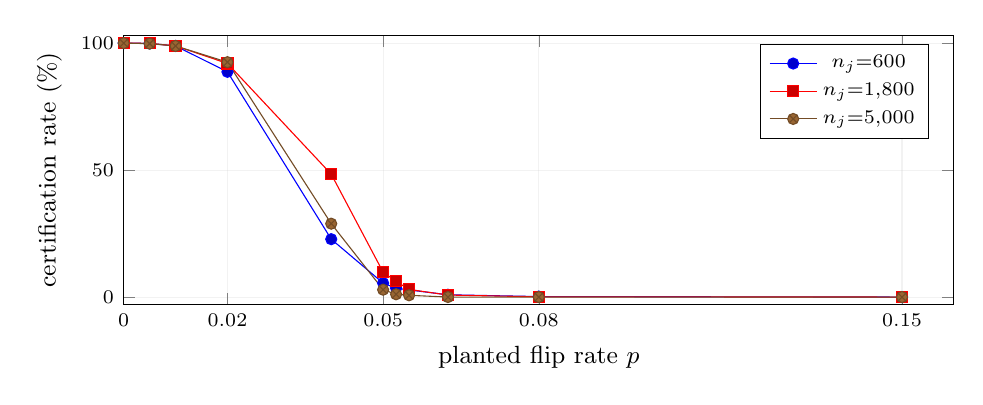
\begin{tikzpicture}
\begin{axis}[width=\linewidth, height=5cm, xlabel={planted flip rate $p$},
  ylabel={certification rate (\%)}, xmin=0, xmax=0.16, ymin=-3, ymax=103,
  label style={font=\small}, tick label style={font=\scriptsize},
  xtick={0,0.02,0.05,0.08,0.15},
  xticklabel style={/pgf/number format/fixed},
  legend pos=north east, legend style={font=\scriptsize}, grid=major,
  grid style={opacity=0.2}]
\powerplots
\end{axis}
\end{tikzpicture}
\caption{Calibration power at $\alpha{=}0.05$ (presented-cells estimand,
$2{,}000$ trials per point). Certification rises smoothly as $p$ falls
below $\alpha$ and is small but nonzero just above it. There the
realized population rate of a planted stratum often falls below
$\alpha$, and certifying it is correct. The unconditional rate of
certificates whose realized error exceeds $\alpha$ stays at or below
\calUnsafeWorst\ in every configuration, against the nominal
\calNominalDelta. The $n_j{=}1{,}800$ curve sits above the other two at
intermediate $p$, because the exact bound's finite-population correction
tightens as the sampled fraction grows. The six-look schedule reaches
most of an $n_j{=}1{,}800$ stratum but a minority of an $n_j{=}5{,}000$
one. The $n_j{=}600$ stratum's final look is the whole stratum, which
cannot certify, so its deepest certifying look is its fourth.}
\Description{Line plot of certification rate against the planted flip
rate for three stratum sizes. Every curve certifies always when the
planted rate is zero, falls towards zero as the planted rate reaches
the budget, and stays near zero above it; the middle stratum size
traces the highest curve at intermediate planted rates.}
\label{fig:power}
\end{figure}
\keeprunin
\paragraph{The planted study.} The study of \secref{sec:exp-validity}
plants flip rates $p \in \calPRange$ at stratum sizes
$\{600, 1{,}800, 5{,}000\}$ and budgets $\alpha \in \{\calAlphaGrid\}$,
in both modes, with $2{,}000$ trials per configuration. The worst rate
of unsafe certificates, \calUnsafeWorst\ (95\% CI \calUnsafeWorstCi),
occurs at $\alpha{=}\calUnsafeWorstAlpha$, $p{=}\calUnsafeWorstP$,
$n_j{=}\calUnsafeWorstSize$, in the \calUnsafeWorstEstimand\ mode. The
presented-cells rate, which leaves out the sampled flips, exceeds
$\alpha$ in at most \calUnsafePresentedWorst\ of runs. Of the
configurations, \calTightNulls\ are planted just above the budget, at
$1.05$ to $1.25$ times $\alpha$, where the futility rule often cannot
dispose of the stratum at the first look and the sampling fraction
climbs. Over these the unsafe rate averages \calUnsafeTightMean. Their
certification rate reaches \calTightCertWorst, and most of those
certificates are correct. At $p$ just above $\alpha$ the realized count
of a planted stratum falls at or below the budget in a large share of
trials, and the exact bound certifies what is actually there. The
reuse-set rate evaluated on default-mode certifications fluctuates past
$\alpha$ in frontier configurations. The worst is \calWorstReuseMetric\
of certified runs at $p{=}\calWorstP$, $\alpha{=}\calWorstAlpha$,
certified \calWorstCertRate\ of the time. That is expected, since the
default mode does not certify that metric. The strict mode holds its own
guarantee within $\delta_j$, with unsafe certificates in at most
\calUnsafeStrictWorst\ of runs.

\keeprunin
\paragraph{The least favorable population.} Fix a stratum of $N$ cells
of which $M$ flip. Under the pinned schedule the certifier's decision at
each look is a threshold on the flips seen so far. It certifies if the
count is at most the largest count whose bound clears the budget (a look
that takes the whole stratum cannot certify). It stops for futility if
the sample's rate exceeds the budget, and otherwise it goes on. The
flips among each look's new cells are hypergeometric given the flips
already seen. The probability of certifying is therefore a finite sum
over the paths of cumulative counts, which the released script
evaluates exactly, with the thresholds of the released certifier.

That probability does not increase with $M$. Take two populations that
differ in one cell, a flip in the larger and none in the smaller, and
sample both by one shuffle. At every look the larger population's sample
holds at least as many flips. A path of counts that certifies still
certifies when every count is lowered: lower counts pass every
threshold the path passed and trip no futility stop that it did not.
Every shuffle that certifies the larger population therefore certifies
the smaller one. In the default mode a certificate is unsafe exactly
when $M > \alpha N$, so its probability is largest at
$M = \lfloor \alpha N \rfloor + 1$, one flip past the budget. In the
strict mode the unsafe event depends on the look, and the script finds
the worst $M$ by scanning. Table~\ref{tab:boundary} gives the result
for each combination of the grid. The script also cross-checks one
combination per budget by running the released certifier on shuffled
populations.

\begin{table}[t]
\caption{The exact probability of an unsafe certificate at the least
favorable fixed population, for each budget and stratum size of the
calibration grid (per-stratum $\delta_j{=}\calNominalDelta$; values
rounded up).}
\label{tab:boundary}
\centering\small
\setlength{\tabcolsep}{4pt}
\input{\paperroot/tableboundary}
\end{table}

\FloatBarrier
\keepheading
\section{The budgets and the strict mode in detail}
\label{app:strict}
\begin{table*}[t]
\caption{What each budget tolerates and what it buys. Tolerated cells
are $\alpha$ times the \deployFalseStratum\ cells of the corpus-scale
cached-FALSE stratum, also given as a multiple of the
\deployTrueStratum\ rows the column marks TRUE. The corpus-scale
columns are the live September certification of
Table~\ref{tab:deploy}. The last six columns give the certification
rate and the mean savings of the formatting-only edit, in percent over
\bootB\ replications: on the Boolean column in both modes, and on the
select column in the default mode (Table~\ref{tab:main};
Appendix~\ref{app:strict}).}
\label{tab:budgets}
\centering\small
\setlength{\tabcolsep}{4pt}
\input{\paperroot/tablebudgets}
\end{table*}
Table~\ref{tab:strict} sets the strict mode beside the default mode on
the configurations of Table~\ref{tab:main}, at the three budgets where
either certifies. The pattern of \secref{sec:exp-main} holds
throughout. Where a stratum's flip rate is well below the budget the
two modes agree, as on the three SO edits at $\alpha{=}0.2$. One budget
step before the default mode's own frontier the strict mode's savings
fall away: on the synonym and scope-widening edits at $\alpha{=}0.1$,
and on both Djinni edits at $\alpha{=}0.2$. The strict mode
issues unsafe certificates too, at a rate the theorem allows. Counted
per stratum, they occur in \strictUnsafeConfigs\ configurations of the
table, most often on \strictUnsafePair\ at
$\alpha{=}\strictUnsafeAlpha$, in \strictUnsafeRate\ of replications.
Each rate sits inside its column's per-stratum level, $\delta_j{=}0.05$
on the Boolean columns and $\delta_j{=}0.025$ on the select column.

\begin{table}[t]
\caption{The default and strict modes on the five edit pairs:
certification rate and mean savings over \bootB\ replications, in
percent. Column \emph{unsafe} is the share of all replications in which
the strict mode issues an unsafe certificate, counted per stratum: one
for a stratum whose realized flip count exceeds $\alpha$ times the cells
it reuses, the event Theorem~\ref{thm:valid} bounds in that mode.}
\label{tab:strict}
\centering\footnotesize
\setlength{\tabcolsep}{4pt}
\input{\paperroot/tablestrict}
\end{table}

\FloatBarrier
\keepheading
\section{The baselines in detail}
\label{app:baselines}
\keeprunin
\paragraph{B1 and B2.} On the formatting edit the similarity score's
entire range is \simLo--\simHi, because shared row text dominates. The
aggregate-only arm runs the same schedule and budgets as the pinned
procedure. On the formatting edit it \aggTightCertF\ at $\alpha{=}0.1$
(\aggFtSavings\ savings, \aggFtRealized\ aggregate error) while the
reused cached-TRUE subgroup carries \aggFtSubgroup\ error. On the
widening edit it \aggTightCertW\ at $\alpha{=}0.1$ and certifies
\aggWsavings\ at $\alpha{=}0.2$ with \aggWsubgroup\ subgroup error. The
effect is not an artifact of giving the baseline a shorter schedule.

\keeprunin
\paragraph{B2$'$: how the competitor was matched.} We matched the
competitor to \sivm{} on every axis we could: the same number of oracle
calls, identical labels, identical error target, the same exact bound
on the selected population, the same total failure probability
$\delta$, and the same reported quantity. Each method's $\delta$ is
split across the number of tests its own procedure performs: \sivm{}
across the Boolean column's two strata and six looks, $\hhSivmPerTest$
per test; the competitor across its candidate thresholds,
$\hhValuePerTest$. The reported quantity is the error among reused
cells, not the presented-cells rate \sivm{} certifies. Run instead on
each stratum separately at $\delta/K$ with a single look, the
competitor would be the non-adaptive special case of \sivm{} itself.

At $\alpha{=}0.2$ on the formatting edit the competitor reused
\hhSupgReused\ cells to \sivm{}'s \hhSivmReused\ from the same
\hhBudget\ labels. At \hhSupgErr\ realized error it satisfies the
bound it was given, against \sivm{}'s \hhSivmErr. On the widening edit
the same pattern holds: \hhSupgReusedW\ reuses at \hhSupgErrW\ versus
\hhSivmReusedW\ at \hhSivmErrW. The extra volume is drawn from the
volatile stratum, \hhSupgTrueRows\ cached-TRUE cells on the formatting
edit and \hhSupgTrueRowsW\ on the widening edit. With the cached value
as the proxy there are only three candidate thresholds, and at
$\alpha{=}0.2$ the aggregate bound clears at the loosest one. The arm
therefore selects \hhSupgSelFrac\ of the rows it was allowed to on the
formatting edit and \hhSupgSelFracW\ on the widening edit. Matched this
way, the competitor reduces to B3, reuse everything, with a certificate
attached. Its bound is satisfied, its aggregate error is real, and its
behavior is indistinguishable from the guarantee-free status quo.

\keeprunin
\paragraph{B2$'$: two caveats.} First, the cached value is the proxy
the reduction names, and the result does not depend on that choice. Run
instead with an embedding-interaction proxy, and with its much larger
threshold search corrected accordingly, the competitor certifies in
\hhEmbCertCells\ of the \hhEmbCells\ (edit, budget) configurations and
lands in the same place. At $\alpha{=}0.2$ on the formatting edit it
reuses \hhEmbReused\ cells at \hhEmbErr\ error, \hhEmbTrueRows\ of them
cached-TRUE cells that flip at \hhEmbTrueErr. On the widening edit it
reuses \hhEmbReusedW\ at \hhEmbErrW, \hhEmbTrueRowsW\ of them
cached-TRUE cells at \hhEmbTrueErrW. The proxy changes how much the
competitor reuses, not where its errors land. Second, with the
cached-value proxy the competitor's per-test level is looser than
\sivm{}'s, because it runs fewer tests. The embedding arm, tested at a
stricter level than \sivm{}'s, still reuses more than \sivm{} at
$\alpha{=}0.2$, so that advantage does not rest on the looser level. The
comparison is matched on the quantity a user sets ($\delta$ in total),
not on the level of any individual test.

\keeprunin
\paragraph{B3: the threshold sweep.} The cells the embedding-transfer
baseline reuses at $\tau{=}0.95$ flip at \flipSoFormatting\ on the
formatting edit and at \bThreeErrW\ on the widening edit, where the
population rate is \flipSoWidening. A sweep of $\tau$ over the per-row
similarities shows the baseline collapsing within a threshold window
about $0.03$ wide. On the formatting edit it falls from \tauFmid\ of
rows reused at $\tau{=}0.96$ to \tauFhi\ at $0.98$ and none at $0.99$.
On the widening edit it falls from \tauWmid\ at $0.94$ to \tauWhi\ at
$0.96$ and none at $0.97$. The realized error among reused rows stays
at the population flip rate at every operating point
(\tauFerrLo--\tauFerrHi\ and \tauWerrLo--\tauWerrHi). The threshold
controls volume, never error, because cross-version similarity carries
no per-cell flip signal (B1).
\par

\FloatBarrier
\keepheading
\section{Further tables}
\label{app:tables}
Five tables the article cites are printed here.

\keeprunin
\paragraph{Models and the headline pair's flip rates.}
Table~\ref{tab:models} lists every model the article uses, by gateway
identifier, with the gateway's list prices. Table~\ref{tab:rates}
reconciles the flip-rate figures quoted for the headline pair and its
cached-TRUE stratum (\secref{sec:exp-setup}).

\keeprunin
\paragraph{The remaining pairs on further models.}
Table~\ref{tab:fampairs} extends the model study of
\secref{sec:exp-families} to the three edit pairs that
Table~\ref{tab:fam} does not cover.

\keeprunin
\paragraph{The benchmark's edit pairs.}
Table~\ref{tab:pairs} transcribes the five versioned prompt-edit pairs
of the benchmark (\secref{sec:benchmark}) from the stored prompt
templates.

\keeprunin
\paragraph{Neighboring systems compared.}
Table~\ref{tab:related} sets \sivm{} against the lines of work it
borrows from, is compared with, or could be mistaken for, by the
quantity each certifies and the axis of change it holds fixed
(\secref{sec:related}).

\begin{table*}[t]
\caption{Every model the article uses, by gateway identifier, with the
gateway's list prices as fetched on \priceFetchedAt.}
\label{tab:models}
\centering\footnotesize
\input{\paperroot/tablemodels}
\end{table*}

\begin{table*}[t]
\caption{Reconciliation of the flip-rate figures quoted for the
headline pair on the evaluation vector and for its cached-TRUE stratum.
Each is a different quantity, a different instrument on the same
quantity, or the same instrument on an earlier draw; none is a
restatement of another.}
\label{tab:rates}
\centering\footnotesize
\renewcommand{\arraystretch}{1.2}
\input{\paperroot/tablerates}
\end{table*}

\ifnum\famPairsAvailable=1\relax
\begin{table*}[t]
\caption{The remaining three edit pairs on further models (same
protocol and same entries as Table~\ref{tab:fam}). Floors are each
model's self-flip rate on that column, measured in the same run; the
primary model's select-column floor is the $n{=}200$ probe of the
noise-floor paragraph. The primary row repeats Table~\ref{tab:main}.
Its widening-column floor is not shown, because the primary model's
self-flip rate under the production column's first version was not
measured (the lab column's \floorBool\ is under the widened
definition).\famPairsSmallStrataNote}
\label{tab:fampairs}
\centering\scriptsize
\setlength{\tabcolsep}{3pt}
\input{\paperroot/tablefampairs}
\end{table*}
\fi
\begin{table*}[t]
\caption{The five versioned prompt-edit pairs. Deltas are transcribed
from the stored prompt templates; referenced fields are the row
attributes the template interpolates. Flip rates are single-fresh-draw labels
against the cached version on the $n{=}\benchN$ evaluation vector
(Table~\ref{tab:main}); the SO synonym pair is measured against the
formatting version's cells (v2$\to$v3), as the benchmark defines it.}
\label{tab:pairs}
\centering\small
\renewcommand{\arraystretch}{1.2}
\begin{tabular}{@{}>{\raggedright\arraybackslash}p{2.1cm}>{\raggedright\arraybackslash}p{3.6cm}>{\raggedright\arraybackslash}p{8.6cm}r@{}}
\toprule
Pair & Column (corpus; contract; referenced fields) & Exact delta & flip \\
\midrule
SO formatting-only (v1$\to$v2) & Data-platform specialist, lab replica (SO; Boolean; role, databases, platforms, tools, other tech) & Two paragraph breaks inserted after the question and before the ``Judge from'' sentence; ``OR heavy analytics engineering'' lowercased to ``or heavy analytics engineering''; no content word changed & \flipSoFormatting \\
SO synonym rewording (v2$\to$v3) & same & ``this person'' $\to$ ``this individual''; ``works primarily on'' $\to$ ``chiefly builds and maintains''; ``heavy analytics engineering'' $\to$ ``intensive analytics engineering''; ``Judge from role \ldots and other tech'' $\to$ ``Decide using their role \ldots and other technologies''; ``Working with multiple \ldots counts as evidence'' $\to$ ``Experience with several \ldots is supporting evidence'' & \flipSoSynonym \\
SO scope widening (v1$\to$v2) & Data-platform specialist, production column (SO; Boolean; same fields) & Definition extended from ``warehouses, lakes, pipelines, distributed data stores, or ML data tooling'' by ``OR heavy analytics engineering''; the exclusion ``Merely using one relational database for app work does not qualify'' replaced by the inclusion ``Working with multiple analytical/distributed databases (BigQuery, Snowflake, Spark, Kafka, Elasticsearch) counts as evidence'' & \flipSoWidening \\
Djinni formatting-only (v1$\to$v2) & Seniority tier, lab (Djinni; four-way ordinal select; position, years of experience, CV text) & The one-line template broken into a question line, three labeled input lines (Position, Years of experience, CV), and the instruction sentence, with no word changed & \flipDjFormatting \\
Djinni criteria change (v2$\to$v3) & same & Sentence appended: ``Evidence of team or people leadership (leading engineers, owning hiring, running a team) moves the candidate up one tier'' & \flipDjCriteria \\
\bottomrule
\end{tabular}
\end{table*}

\begin{table*}[t]
\caption{What neighboring systems certify, and across what. \sivm{} is
the only row whose certified quantity is the reuse of cached outputs
across a change of the prompt definition.}
\label{tab:related}
\centering\small
\renewcommand{\arraystretch}{1.2}
\begin{tabular}{@{}>{\raggedright\arraybackslash}p{3.1cm}>{\raggedright\arraybackslash}p{4.0cm}>{\raggedright\arraybackslash}p{2.6cm}>{\raggedright\arraybackslash}p{3.2cm}>{\raggedright\arraybackslash}p{2.7cm}@{}}
\toprule
System or line & Certified quantity & Held fixed & Changes & Guarantee form \\
\midrule
SUPG, ABae, BARGAIN, LOTUS, ThalamusDB, Task Cascades~\cite{supg,abae,bargain,lotus,thalamusdb,taskcascades} & precision, recall, or accuracy of one query's answer against an oracle & the query definition & nothing (one-shot execution) & finite-sample bound per query \\
vCache~\cite{vcache} & correctness of serving a cached answer to a \emph{new} query & the answer semantics & the incoming query & learned per-entry threshold at a user error rate \\
FreshCache, Evergreen~\cite{freshcache,evergreen} & probability that a cached entry is stale (world drift); cost of verifying aggregates & the query definition & the world the answer describes & fitted staleness model per tier; confidence sequences \\
Stale-view cleaning, online aggregation~\cite{svc,ola} & error of an answer served from a stale view; a running aggregate & the view definition & the base data & sampling bound on the answer \\
Classical incremental view maintenance (IVM)~\cite{dbsp} & exact equality of the maintained view with recomputation & the view definition & the base data & algebraic (no sampling) \\
View adaptation after redefinition~\cite{gupta95} & exact equivalence of the rewritten view & deterministic operators & the view definition & algebraic (no sampling) \\
Step-level reuse~\cite{stepcache} & per-step equivalence under a perturbed request & the model & the request & deterministic per-step check \\
Guarantee-free semantic caches~\cite{gptcache} (B3) & nothing: a hit is a similarity above a threshold & nothing & the incoming query & none \\
Per-output verification: assertions~\cite{spade}, regression suites~\cite{retain}, majority vote~\cite{selfconsistency} & correctness of one output against a checker or a majority & the prompt & the output under test & per-output check, no population bound \\
Conformal and distribution-free risk control for model outputs: risk-controlling prediction sets, Learn then Test~\cite{rcps,ltt} & a risk of one fixed predictor's outputs on new inputs & the predictor (model and prompt) & the input & finite-sample bound from a held-out calibration set \\
\sivm{} (this work) & false-reuse rate of cached stochastic cells kept under the new definition, per stratum & the model snapshot and the data & the prompt definition & exact finite-sample bound per stratum and look \\
\bottomrule
\end{tabular}
\end{table*}


\EOD

\end{document}
